\documentclass{article}
\usepackage[margin=0.75in]{geometry}
\usepackage{graphicx}
\usepackage{hyperref}
\usepackage{subcaption}
\usepackage{boxedminipage}

\begin{document}

    \title{\vspace{-3em}
        Machine Learning Engineering Nanodegree \\
        \large Capstone Project Report \\
        \huge ChestR \\
        \large Disease Predictor for Chest \\
        X-Rays} 
    \author{Shishir Horane}
 
    \maketitle 

    \section{Project Overview}

    In medical industry chest x-ray is the most commonly performed diagnostic x-ray examination. It produces images of the heart, lungs, airways, blood vessels and the bones of the spine and chest. An x-ray(radiograph) is a non-invasive medical way for physicians to diagnose and treat medical conditions. Performing such an x-ray involves exposing the the chest to a small dose of ionizing radiation to produce the pictures of the body. X-rays are the most frequently used form of medical imaging. 
    
    The chest x-ray is commonly the first imaging test used to help diagnose symptoms such as chest pain, breathing difficulties, bad or consistent cough etc. Physicians will use these imaging to diagnose or monitor treatments for conditions such as pneumonia, heart problems, lung cancer, fluid or air collection in lungs etc. Although this isn't necessarily a conclusive diagnosis for all kind of diseases it is the first tool of diagnosing any possible illnesses for the above said symptoms.\cite{xray-details} 

    This project will showcase a neural network which will provide the predictions on chest X-ray images with some certainty better than random guessing. 

    \section{Problem Statement}
    Chest X-ray exams are one of the most frequent and cost-effective medical imaging examinations available. However, clinical diagnosis of a chest X-ray can be challenging and sometimes more difficult than diagnosis via chest CT.\cite{nih-kaggle}
    
    Reading and diagnosing chest x-ray images may be a relatively simple task for radiologists but, in fact, it is a complex reasoning problem which often requires careful observation and knowledge of anatomical principles, physiology and pathology. Such factors increase the difficulty of developing a consistent and automated technique for reading chest X-ray images while simultaneously considering all common thoracic diseases.\cite{nih-gov-xray-release}

    There is a need to develop an automated technique that could analyze a given chest x-ray and which could predict the possible common thoracic diseases with some certainty. Also, it should aid radiologists or physicians by highlighting the suspected common areas of disease in order to pay close attention to certain areas of a chest x-ray, so as to not misdiagnose these diseases. This automated technique could benefit patients in developing countries who do not have access to the radiologists to read these x-rays.
    One such success metric of such a system would be the ability to predict disease outcome with some certainty than say, random prediction.

    \section{Data Exploration and Visualization}
    If a dataset is present, features and calculated statistics relevant to the problem have been reported and discussed, along with a sampling of the data. In lieu of a dataset, a thorough description of the input space or input data has been made. Abnormalities or characteristics about the data or input that need to be addressed have been identified.
    
    To that effect National Institutes of Health has released over 112,000 chest X-ray images with the labeled data, 15 labels: 14 diseases, 1 no findings.\cite{nih-gov-xray-release} we will be using this data to build a convolutional neural network for disease prediction from a chest X-ray image. In order to build the neural network the following data analysis was executed on the above said data.

    \begin{figure}
        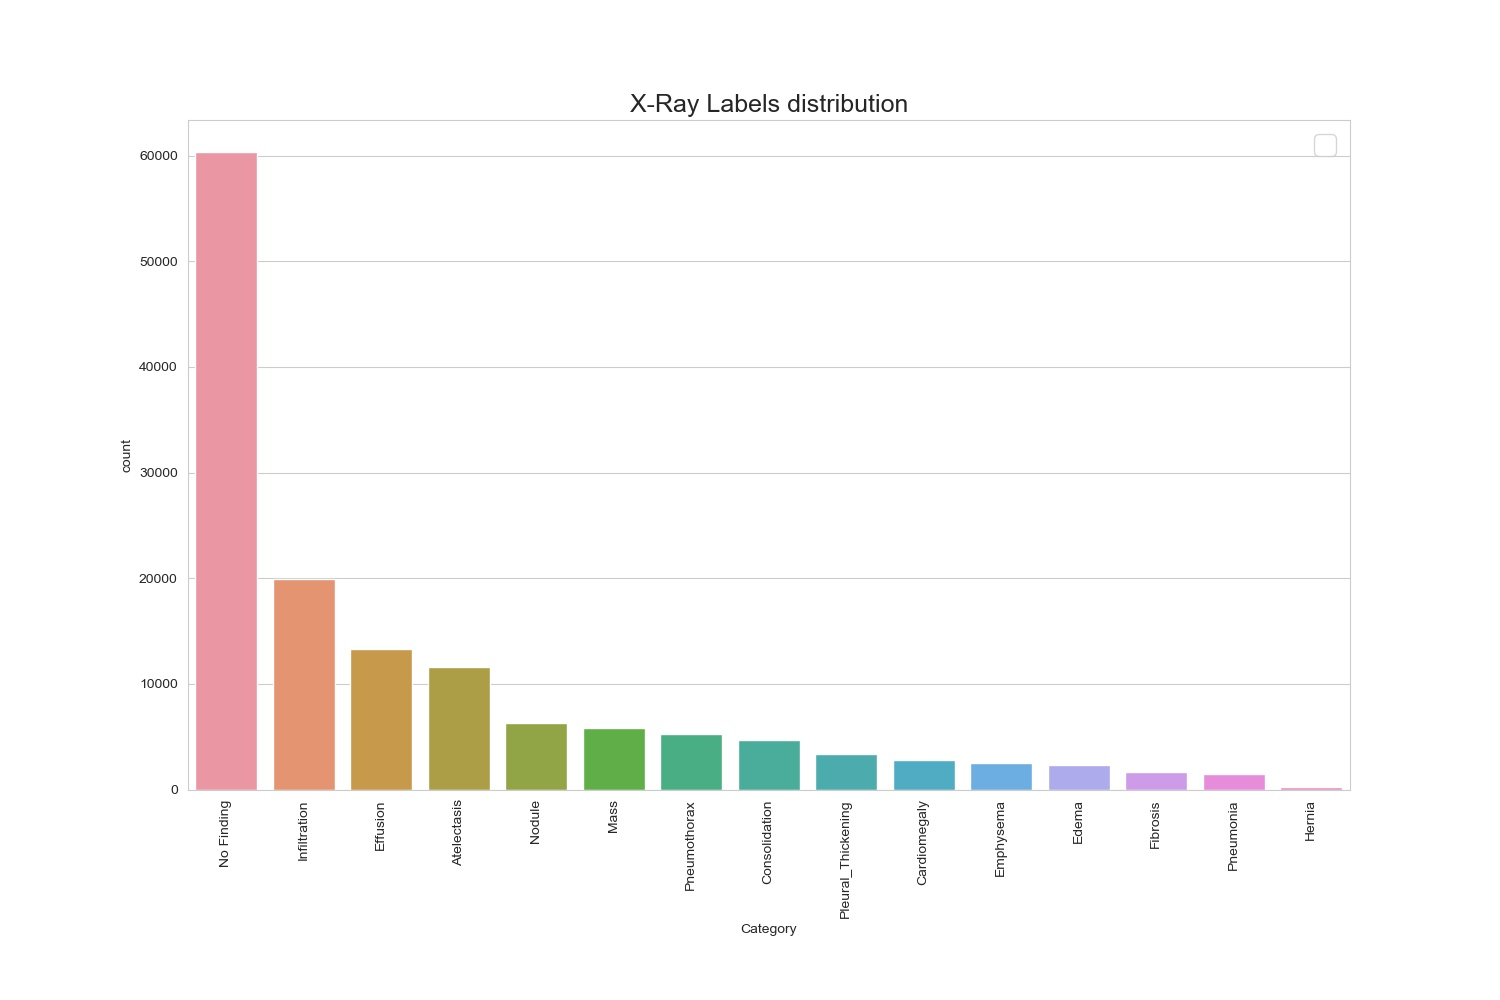
\includegraphics[width=\linewidth]{./images/labels_distribution.jpg}
        \caption{Disease label distribution.}
        \label{fig:labels-distribution}
    \end{figure}
    
    The figure \ref{fig:labels-distribution} shows the distribution of the 112000 X-ray images. It can be seen that our data is highly biased with over 60,000 of chest x-ray images labeled with \textit{No Finding}, and over fifty percent of the images tagged with three diseases \textit{Infiltration, Effusion, Atelectasis}. The rest of the 11 diseases are labeled with the remaining fifty percent of the images. This is an expected data given the nature of healthcare industry where often procedures are performed as a preventative or diagnosing step. And the possiblity of multiple pathologies of similar nature. Given this analysis it is a given that we will need to do some preprocessing to balance the data.

    The figure \ref{fig:labels-vs-gender} shows the disease labels vs gender distribution. The data is more or less simlarly distributed and given the pathologies there is no co-relation between the disease labels and the gender. Thus, it is fine to ignore the gender feature for our analysis.

    \begin{figure}
      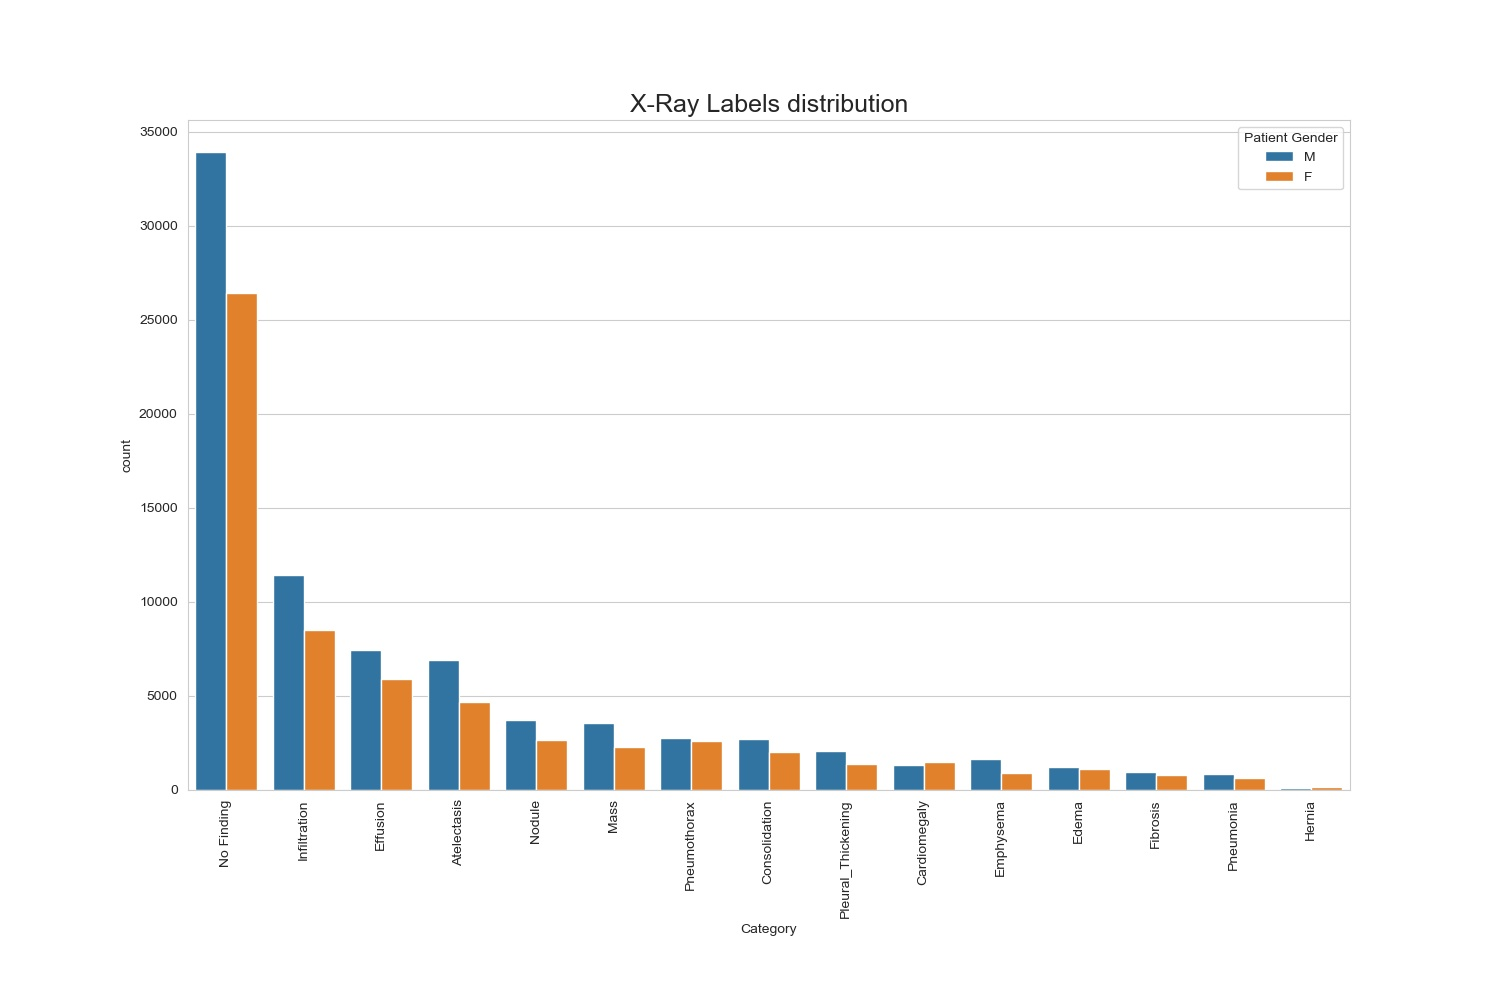
\includegraphics[width=\linewidth]{./images/labels_vs_gender.jpg}
      \caption{Disease labels vs Gender distribution.}
      \label{fig:labels-vs-gender}
    \end{figure}

    The figure \ref{fig:age-vs-gender} shows the gender distribution over the age period. This figure shows that the provided data distribution ranges for all genders for all age periods. This reflects the above conclusion that there is no need for the gender feature to be considered for the analysis.

    \begin{figure}
      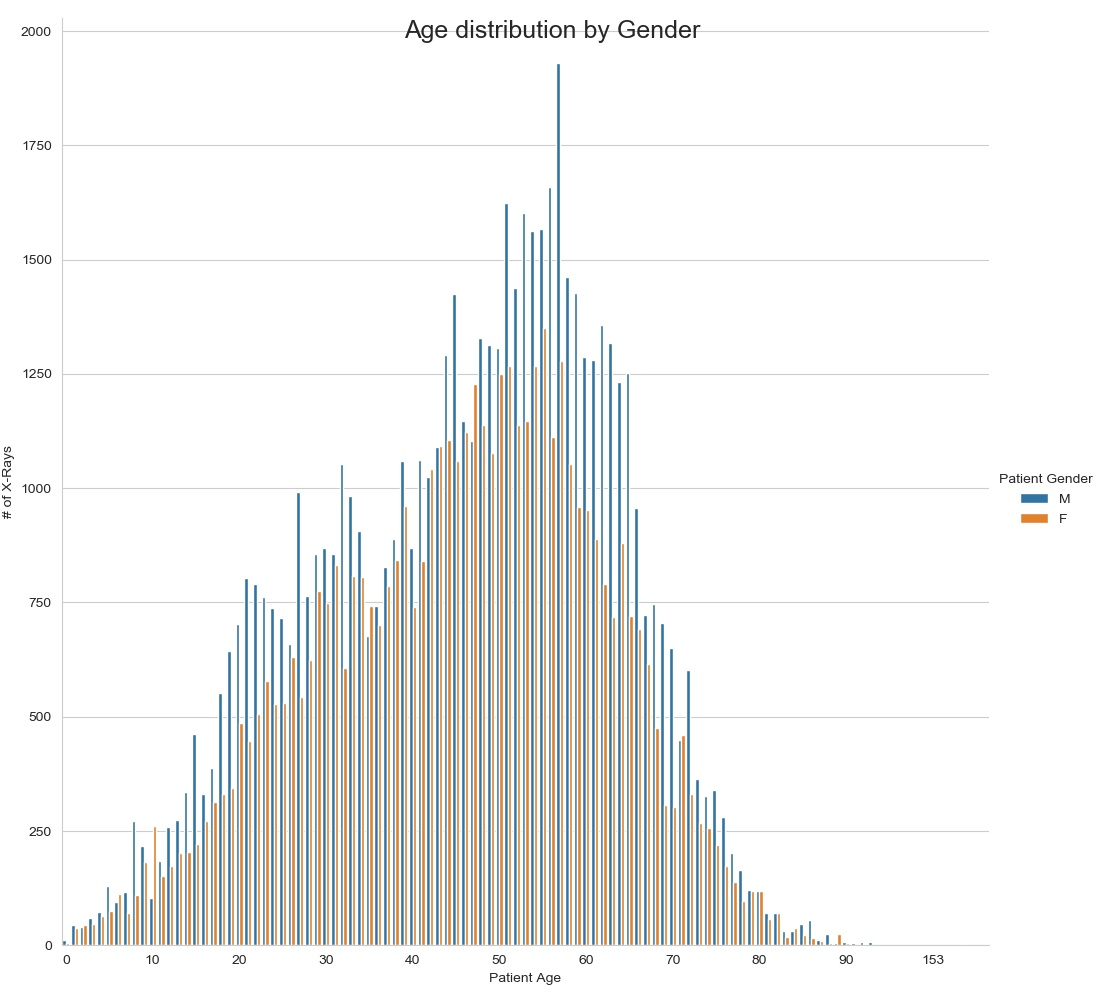
\includegraphics[width=\linewidth]{./images/age_gender_distribution.jpg}
      \caption{Age vs Gender distribution}
      \label{fig:age-vs-gender}
    \end{figure}

    The figure \ref{fig:disease-age-vs-gender} shows the each category of disease labels distribution over gender and age. The data seems to show that all the disease labels are independent of age or gender. This helps us to decide that age feature is not a factor for contribution to the diseases and can be safely ignored for our analysis.

    \begin{figure}
        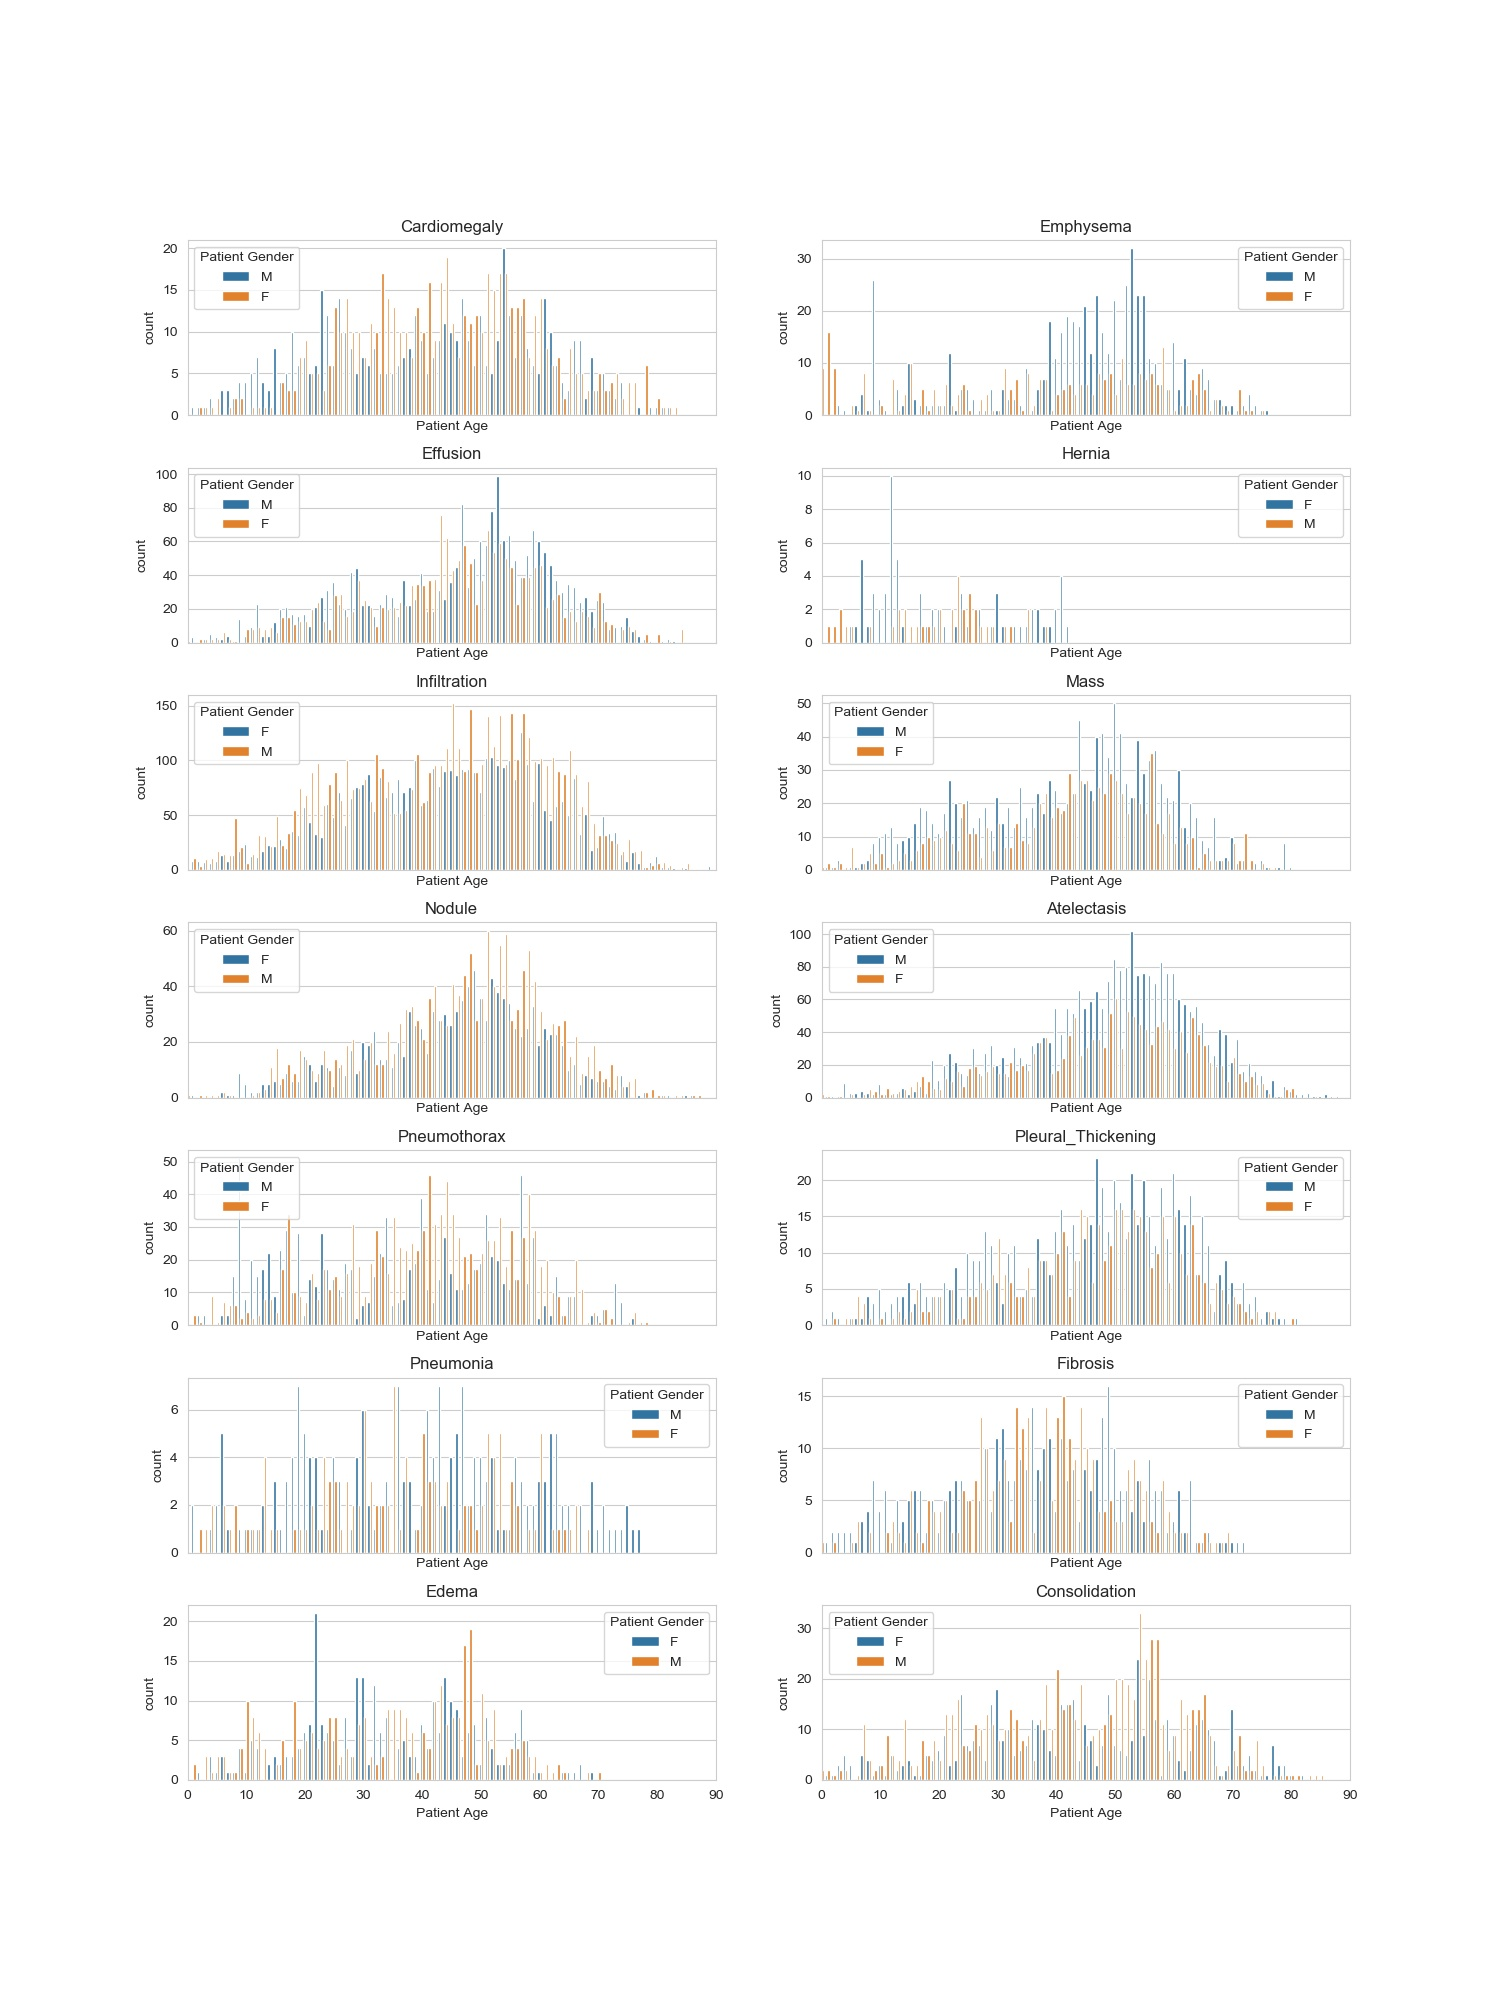
\includegraphics[width=\linewidth]{./images/disease_age_gender_distribution.jpg}
        \caption{Disease vs Age vs Gender distribution}
        \label{fig:disease-age-vs-gender}
    \end{figure}

    The figure \ref{fig:multiple-diseases} shows the classification of diseases by multiple pathologies present in the dataset. It can be seen that most of the data for the labeled data shows some xrays with single disease but a lot more with multiple pathologies. It means our CNN model needs to be able to predict multiple diseases and these disesases are not exclusive to each other.

    \begin{figure}
        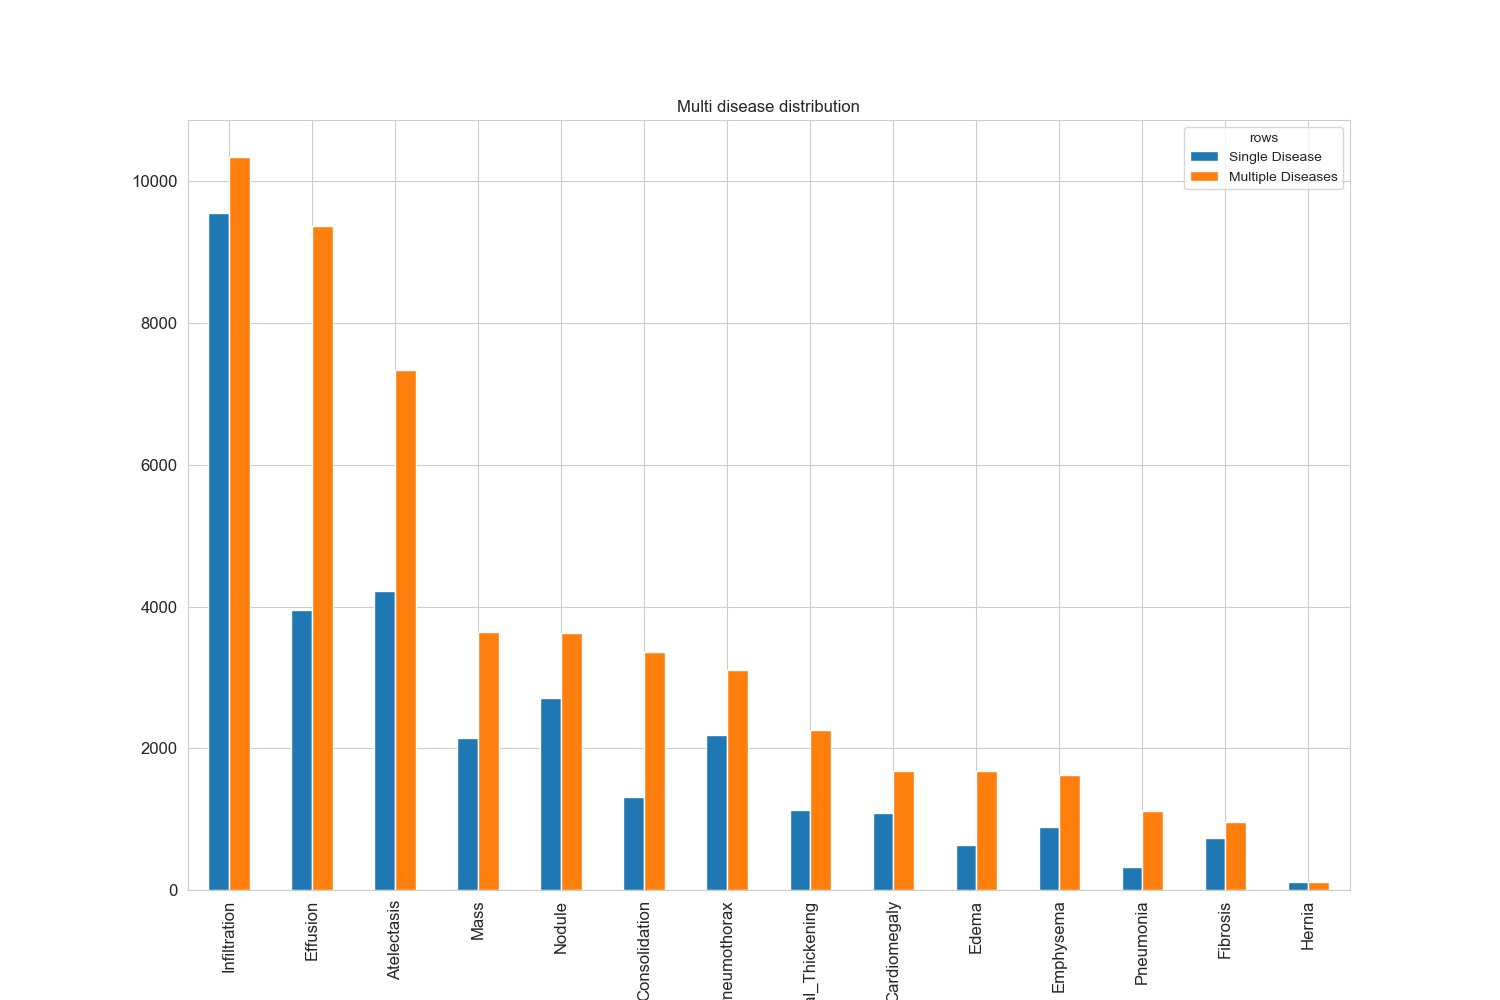
\includegraphics[width=\linewidth]{./images/multiple_disease_distribution.jpg}
        \caption{Multiple pathologies in the dataset}
        \label{fig:multiple-diseases}
    \end{figure}

    \section{Algorithms and Techniques}
    Given the nature of the data, we have a lot of labeled images the general technique to approach such a problem is developing a Deep Neural Network model which would learn the pattern of the diseases in the provided images. Once we develop this learned model it should be able to predict the disease in the chest x-ray images. To that effect the project takes an iterative approach on building the convolutional neural network for disease prediction. In the following subsections we discuss the data preprocessing followed by a benchmark model with analyzed results. Subsequently we will see the development of a convolutional neural network which is further more refined by the applicaitons of transfer learning in deep neural networks. The metrics used for analysis are Receive Operating Curve(ROC) and Area Under the Curve(AUC) for different models. This metric along with the \textit{Precision, Recall and F1-Score} will provide the comparison of the performance of these models. Since the problem statement is to develop a disease predictor and the inherent bias in the data with high number of negative results, ROC is the most appropriate metric to compare the performance characteristics for these models. Finally we see the comparison and evaluation of our most refined model for disease prediction.
    
    \subsection{Data Preprocessing}
    As per the data analysis done in the above section, we get rid of all the features other than the image names and indexes. This is done as part of our \textit{Preprocessing} step.\cite{github-proj}. Following preprocessing is performed on this data:
    \begin{itemize}
        \item Data is loaded from \textit{Data-Entry-2017.csv}, the unnecessary features like \textit{Age, Gender, Original Image width, height, Bounding Box x, y etc.} are deleted. 
        \item Loads all image paths from data folder.
        \item Extract the disease labels and get rid of the label with low count of data, as seen from \ref{fig:labels-distribution} the label \textit{Hernia} has only 227 images which is insufficient to meaningfully predict with the huge bias in remaining data, hence get rid of this prediction label altogether. Thus, the scope of the prediction is narrowed down to the 13 disease labels. 
        \item The dataset is sampled by weight and reduced down to 50000 images, since anything above it is too much data to be meaningfully processed on local machine. The figure \ref{fig:sampled-disease} shows the sampled images by weight, thus still keeping the possible relation with multiple pathologies in the data.
        \item The data is then split into 40000 images for \textit{training}, 6000 images for \textit{validation} and 4000 images for \textit{testing} phases.
        \item The data is co-related with the disease prediction vector with truth values for the disease labels.
    \end{itemize} 
    
    \begin{figure}
        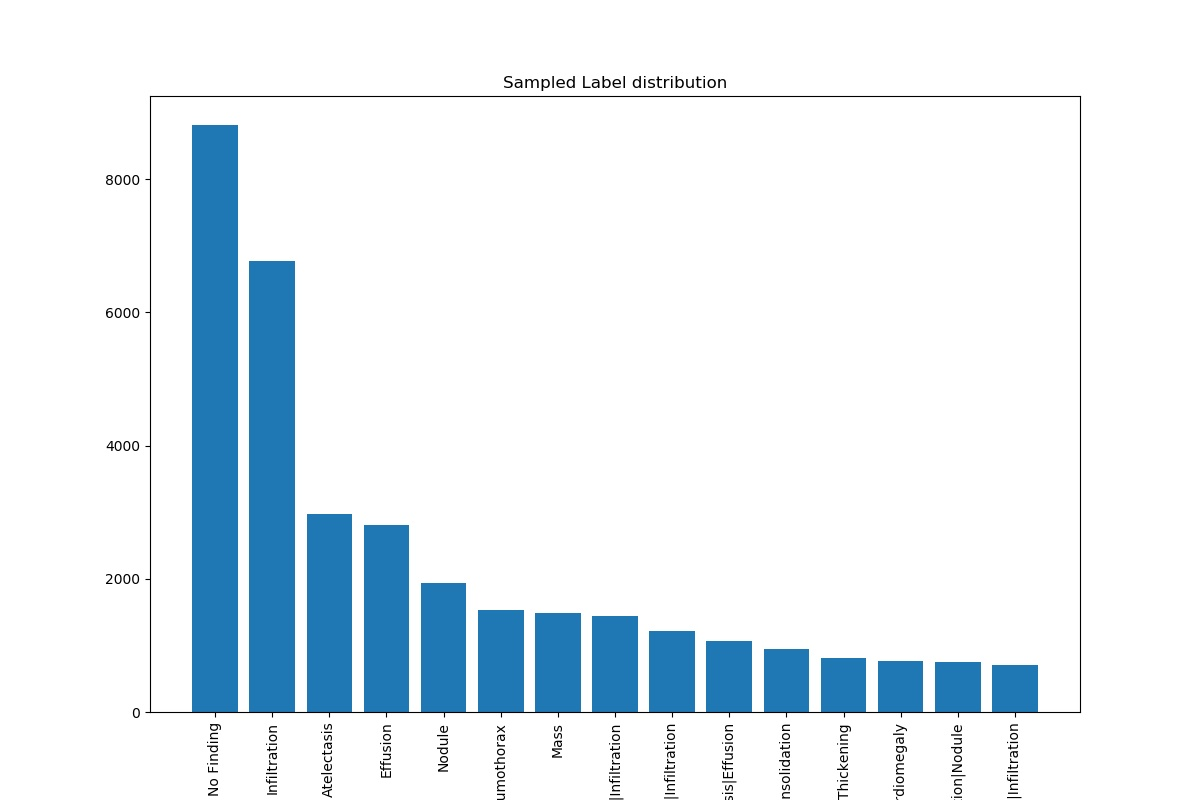
\includegraphics[width=\linewidth]{./images/sampled_disease_distribution.jpg}
        \caption{Sampled by weights}
        \label{fig:sampled-disease}
    \end{figure}

    The text below shows the output from the "pre-processing" stage when loading the data.

    \fbox{\begin{minipage}{\textwidth}
        Loading data. \\
        Total data loaded:  112120 \\
        Loaded paths for images:  112120 \\
        Total Disease labels in dataset: 14 \\
        Disease Labels distribution (14): ('Cardiomegaly', 2776), ('Emphysema', 2516), ('Effusion', 13317), ('Hernia', 227), ('Infiltration', 19894), ('Mass', 5782), ('Nodule', 6331), ('Atelectasis', 11559), ('Pneumothorax', 5302), ('Pleural\_Thickening', 3385), ('Pneumonia', 1431), ('Fibrosis', 1686), ('Edema', 2303), ('Consolidation', 4667) \\
        Cleaned up disease Labels distribution (13): ('Cardiomegaly', 2776), ('Emphysema', 2516), ('Effusion', 13317), ('Infiltration', 19894), ('Mass', 5782), ('Nodule', 6331), ('Atelectasis', 11559), ('Pneumothorax', 5302), ('Pleural\_Thickening', 3385), ('Pneumonia', 1431), ('Fibrosis', 1686), ('Edema', 2303), ('Consolidation', 4667) \\
        Dataset shape after sampling: (50000, 18) \\
        Generating disease prediction vector... \\
        Splitting the data for train and test... \\
        Training set size: (40000, 19) \\
        Validation set size: (6000, 19) \\
        Testing set size: (4000, 19) \\
        Load images and generate dataframes... \\
        Found 112120 images belonging to 12 classes. \\
        Generated data frame with loaded images:  (40000, 19) \\
        Found 112120 images belonging to 12 classes. \\
        Generated data frame with loaded images:  (6000, 19) \\
        Found 112120 images belonging to 12 classes. \\
        Generated data frame with loaded images:  (4000, 19) \\
        Data load complete!
    \end{minipage}}

    Once the data has been preprocessed we can see the sampled images from the dataset in the figure \ref{fig:sampled-xrays}

    \begin{figure}
        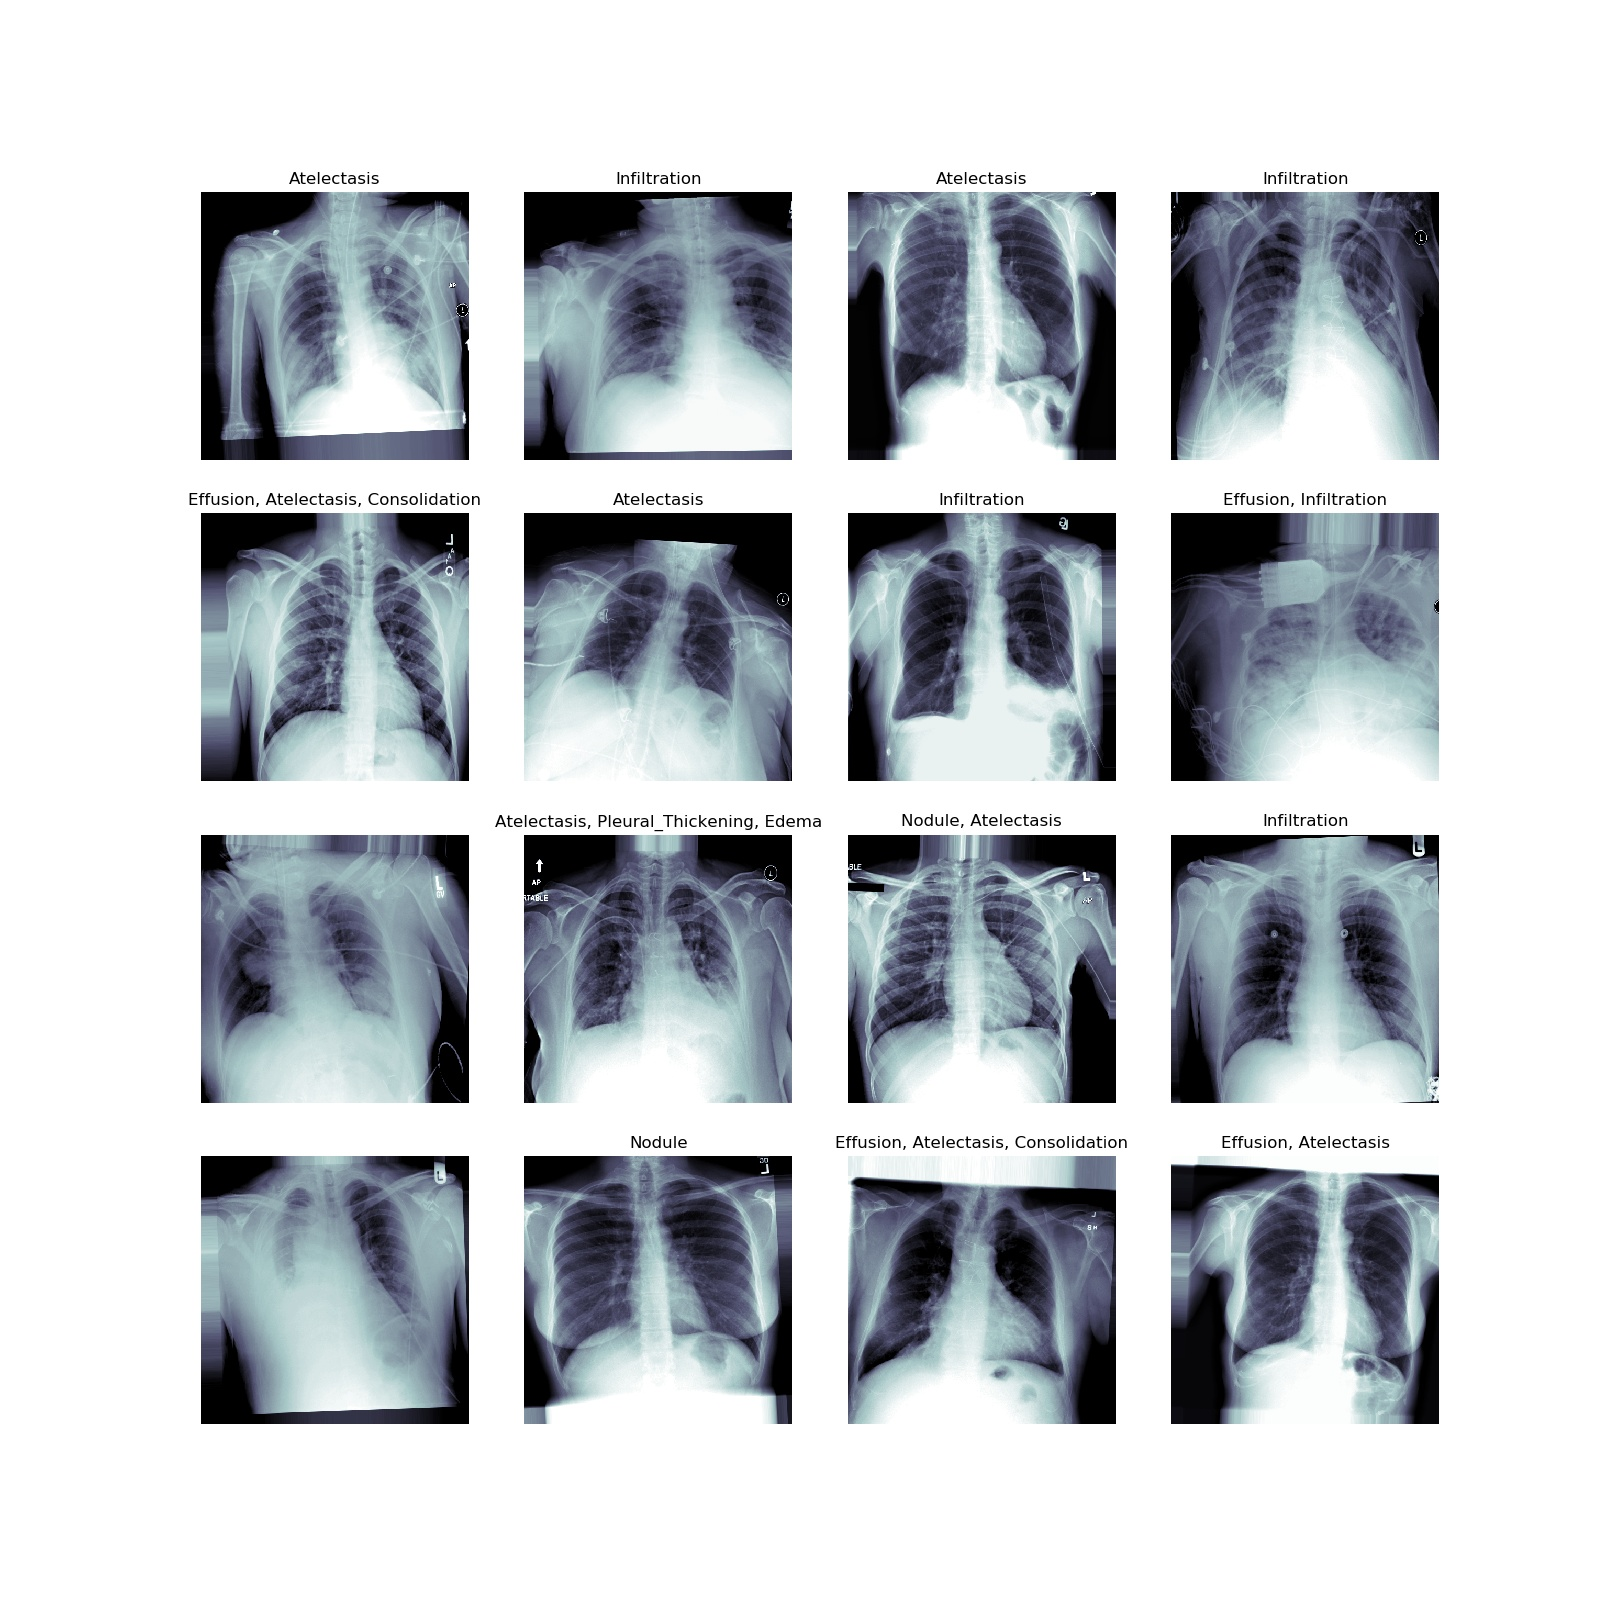
\includegraphics[width=\linewidth]{./images/sampled_loaded_training_set.jpg}
        \caption{Loaded training set samples}
        \label{fig:sampled-xrays}
    \end{figure}

    \subsection{Benchmark - Base model}
    
    As the first step towards building a CNN the first step was to build a Dense MLP with 8 layers. This is our benchmark base model since it is simple to construct and train such a model. Upon analyzing this model we can see that it truly behaves like a random classifier with very low scores on predicting any diseases.

    The text below gives an idea on the layers shape and outputs.

    \fbox{\begin{minipage}{\textwidth}
        =================================================================\\ 
        Layer (type)                 Output Shape              Param \# \\ 
        =================================================================\\ 
        dense\_1 (Dense)              (None, 128, 128, 16)      32 \\ 
        =================================================================\\ 
        dropout\_1 (Dropout)          (None, 128, 128, 16)      0 \\ 
        =================================================================\\ 
        dense\_2 (Dense)              (None, 128, 128, 32)      544 \\ 
        =================================================================\\ 
        dropout\_2 (Dropout)          (None, 128, 128, 32)      0 \\ 
        =================================================================\\ 
        dense\_3 (Dense)              (None, 128, 128, 32)      1056 \\ 
        =================================================================\\ 
        dropout\_3 (Dropout)          (None, 128, 128, 32)      0 \\ 
        =================================================================\\ 
        flatten\_1 (Flatten)          (None, 524288)            0 \\ 
        =================================================================\\ 
        dense\_4 (Dense)              (None, 13)                6815757 \\ 
        ================================================================= \\ 
        Total params: 6,817,389\\ 
        Trainable params: 6,817,389\\ 
        Non-trainable params: 0\\ 
        =================================================================\\ 
    \end{minipage}}

    The above said model was trained on 10 epochs to get the weights. The best weights were stored using \textit{Keras.Model.Checkpoint} and further loaded for analysis. 

    The figure \ref{fig:base-mlp-roc} shows that the ROC curve is a linear line, thereby giving us an AUC of 0.5 across the board on all the 13 prediction labels. It means that this model is truly random and a terrible classifier.

    \begin{figure}
        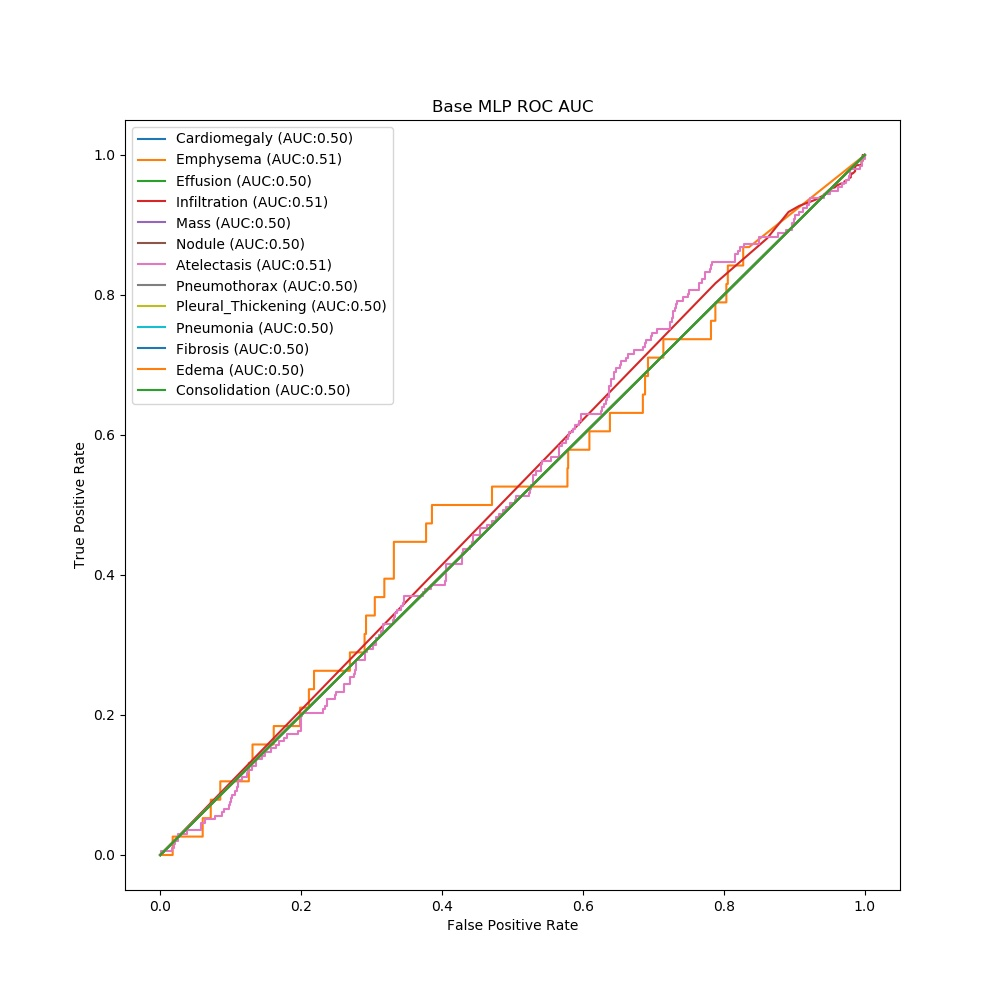
\includegraphics[width=\linewidth]{./images/base_mlp_roc_auc.jpg}
        \caption{Base MLP ROC AUC}
        \label{fig:base-mlp-roc}
    \end{figure}

    Just to double check we can view the sample predictions on the images below in \ref{fig:base-mlp-pred-samples}, which shows that this base model is essentially predicting only one disease \textit{Mass} for every kind of X-Ray.  

    \begin{figure}
        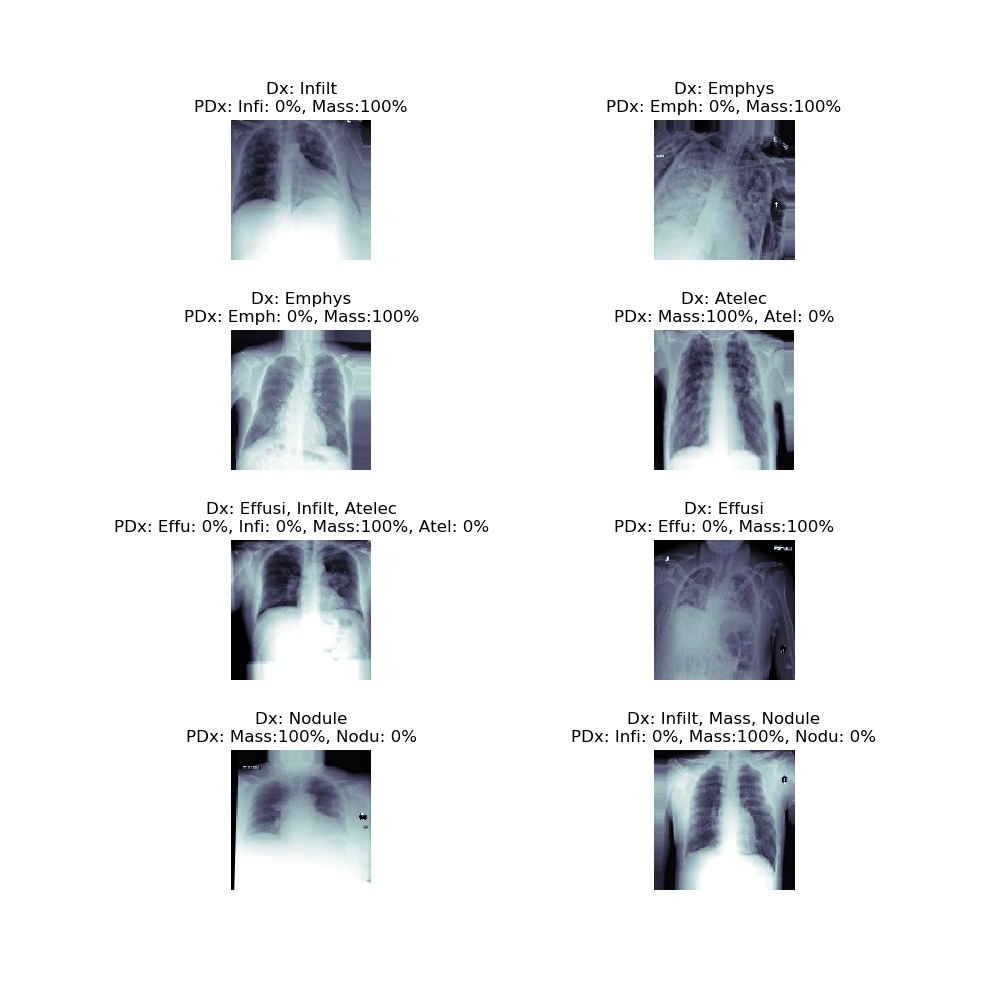
\includegraphics[width=\linewidth]{./images/base-mlp_sample-images-pred-view.jpg}
        \caption{Base MLP Samples with Actual diagnosis vs Predicted Diagnosis}
        \label{fig:base-mlp-pred-samples}
    \end{figure}

    Note: The \textit{base-mlp-neural-net.py} hosts the source code for training this model in the project.\cite{github-proj}

    \subsection{Convolutional Neural Network - Implementation and Troubles}
    With the benchmark model underway, I started implementation of a convolutional neural network for training the dataset on disease predictions. This involved adding different layers and doing some trial and errors. The main problem faced during this phase was getting the model to train on the GPU with tensor flow. The experiments were carried out on Azure Virtual Machine with Nvidia Tesla M60 Graphics card with a memory of 7.5GB, however, while training I was consistently getting "Resource exhausted: OOM error". This meant that the graphics card was running out of memory when building the models. This involved reducing the batch size of the training generators. However, the issue was persistent. After reading about OOM error messages, stack overflow topics, trial and errors it seemed like the size of X-Ray images was the issue. These x-ray images were loaded into the memory on its full size of 1024*1024 pixels. This basically generated a huge datasize for training the designed CNN. On the order of 128Million trainable parameters. After various experiments, it was seen that reducing the image size to 128*128 pixels allowed sufficient memory for the model to be trained on the GPU. 

    \subsubsection{The CNN model and Analysis}
    After the above issues were resolved, and running different trial and errors with varying epoch values ranging from 2 to 100, and tuning with different optimizers following 14 layer CNN model was the best possible outcome of these experiments. 

    \fbox{\begin{minipage}{\textwidth}
        =================================================================  \\ 
        Layer (type)                 Output Shape              Param   \\ 
        =================================================================  \\ 
        conv2d\_1 (Conv2D)            (None, 128, 128, 64)      320  \\ 
        =================================================================  \\ 
        conv2d\_2 (Conv2D)            (None, 128, 128, 64)      16448  \\ 
        =================================================================  \\ 
        max\_pooling2d\_1 (MaxPooling2) (None, 64, 64, 64)        0  \\ 
        =================================================================  \\ 
        conv2d\_3 (Conv2D)            (None, 64, 64, 128)       32896  \\ 
        =================================================================  \\ 
        conv2d\_4 (Conv2D)            (None, 64, 64, 128)       65664  \\ 
        =================================================================  \\ 
        max\_pooling2d\_2 (MaxPooling2 (None, 32, 32, 128)       0  \\ 
        =================================================================  \\ 
        dropout\_1 (Dropout)          (None, 32, 32, 128)       0  \\ 
        =================================================================  \\ 
        conv2d\_5 (Conv2D)            (None, 32, 32, 256)       131328  \\ 
        =================================================================  \\ 
        max\_pooling2d\_3 (MaxPooling2 (None, 16, 16, 256)       0  \\ 
        =================================================================  \\ 
        conv2d\_6 (Conv2D)            (None, 16, 16, 256)       262400  \\ 
        =================================================================  \\ 
        global\_average\_pooling2d\_1 ( (None, 256)               0  \\ 
        =================================================================  \\ 
        dense\_1 (Dense)              (None, 512)               131584  \\ 
        =================================================================  \\ 
        dropout\_2 (Dropout)          (None, 512)               0  \\ 
        =================================================================  \\ 
        dense\_2 (Dense)              (None, 13)                6669  \\ 
        =================================================================  \\ 
        Total params: 647,309  \\ 
        Trainable params: 647,309  \\ 
        Nontrainable params: 0  \\ 
        =================================================================
    \end{minipage}}
    
    

    Note: The source code for this training model can be found in \textit{chestr-cnn-model.py}\cite{github-proj}

    \subsubsection{Transfer Learning - InceptionV3}  
    As can be seen from the above model experiments it seemed like the model was stuck in local minima and couldn't make any more improvements with varying epoch values. Thus I decided to apply "Transfer Learning" technique to my model. I used InceptionV3 pre-trained model with "ImageNet" weights. InceptionV3 is an award winning model trained on ImageNet database for classifying images. Given that we have a high volume of data and the image classes are fairly different between "ImageNet" and Chest X-Ray, I decided to apply the "Transfer learning" principles, i.e. train the whole model with freezing and unfreezing pre-trained models along with my top layer. 

    However, these experiments resulted in failures. The model failed to make any kind of improvements, in fact it kept on miscategorizing data. Another challenge was that the pretrained models require the input data(images) are provided with three channels i.e. RGB. The original processing for the data was done with single channel i.e. 'Grayscale' category, since X-rays are always in a grayscale category. This required the data fixing and read the images as RGB instead of grayscale. The online forums indicated that this would work fine, however the model failed to perform any better than the previously developed CNN model.

    Note: This model's source code is hosted in \textit{chestr-inceptionv3-cnn.py}.

    \subsubsection{Transfer Learning - VGG19}  
    Upon further failures to get desired results, I started experimenting with "Transfer learning" with VGG19 pre-trained models and with "ImageNet" weights. As an experiment I trained all the layers without freezing any layers and the result can be seen in the figure \ref{fig:cnn-vgg19-roc-auc}. The AUC is varying between 0.43 to 0.57 same as the CNN model discussed above. However, if we look at the predicted samples in figure \ref{fig:cnn-vgg19-samples} the prediction probabilities are fairly high for all the diseases. More than 80 percent in most cases. This tells us that this model is overly optimistic and calling every X-ray as a disease with high probabilities. This essentially means this model has \textit{High Recall and Low Precision}. 

    \begin{figure}
        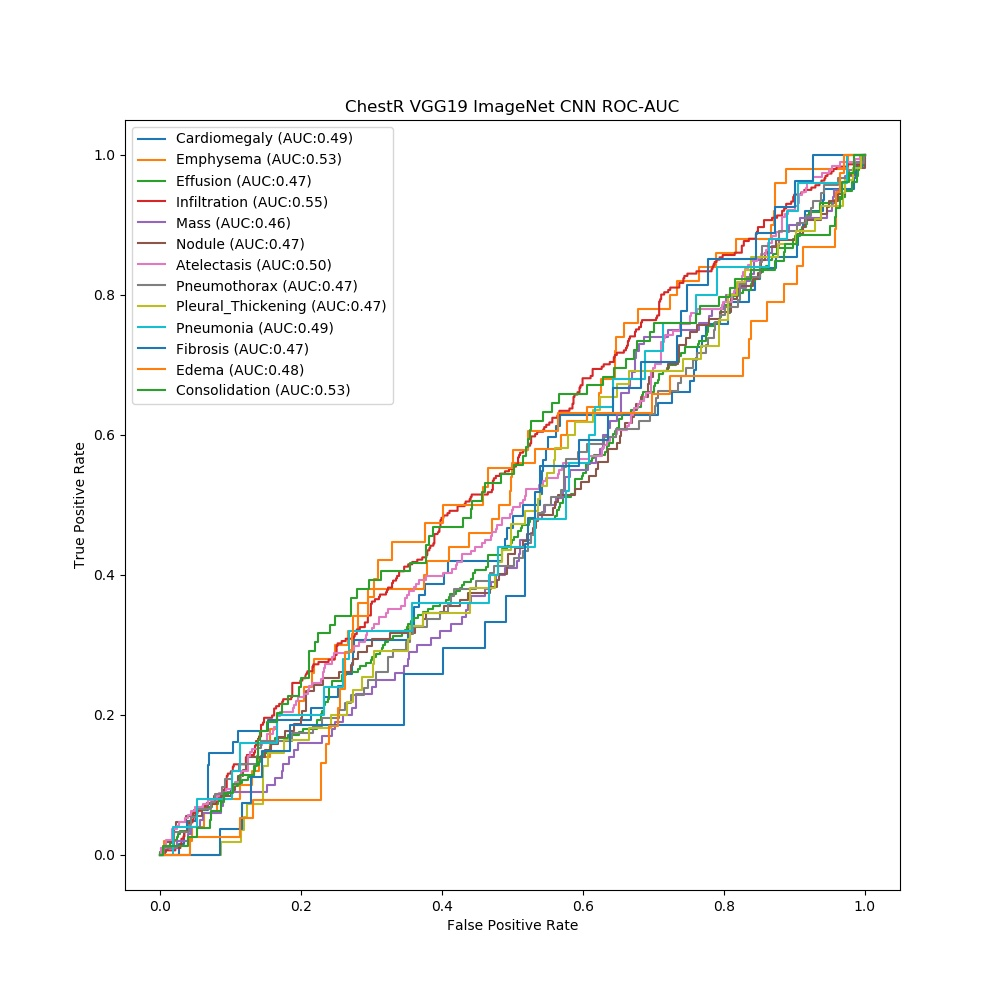
\includegraphics[width=\linewidth]{./images/chestr-vgg19_roc_auc.jpg}
        \caption{ChestR CNN VGG19 ROC AUC}
        \label{fig:cnn-vgg19-roc-auc}
    \end{figure}

    \begin{figure}
        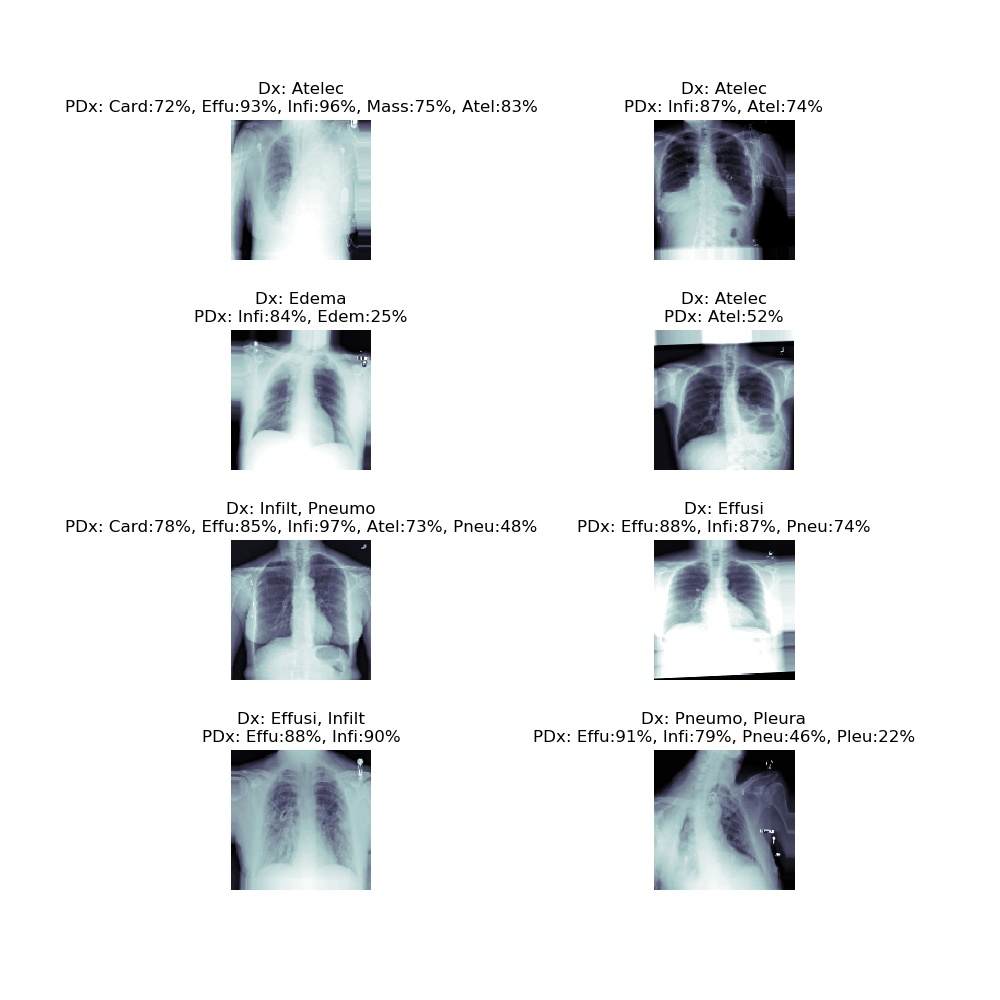
\includegraphics[width=\linewidth]{./images/chestr-vgg19_sample-images-pred-view.jpg}
        \caption{ChestR CNN VGG19 Sample Predictions}
        \label{fig:cnn-vgg19-samples}
    \end{figure}

    The below 32 layer VGG19 pre-trained model with the Convolutional neural network was fully trained to get above results.

    \fbox{\begin{minipage}{\textwidth}
        ================================================================= \\ 
        Layer (type)                 Output Shape              Param \\ 
        ================================================================= \\ 
        input\_1 (InputLayer)         (None, 128, 128, 3)       0 \\ 
        ================================================================= \\ 
        block1\_conv1 (Conv2D)        (None, 128, 128, 64)      1792 \\ 
        ================================================================= \\ 
        block1\_conv2 (Conv2D)        (None, 128, 128, 64)      36928 \\ 
        ================================================================= \\ 
        block1\_pool (MaxPooling2D)   (None, 64, 64, 64)        0 \\ 
        ================================================================= \\ 
        block2\_conv1 (Conv2D)        (None, 64, 64, 128)       73856 \\ 
        ================================================================= \\ 
        block2\_conv2 (Conv2D)        (None, 64, 64, 128)       147584 \\ 
        ================================================================= \\ 
        block2\_pool (MaxPooling2D)   (None, 32, 32, 128)       0 \\ 
        ================================================================= \\ 
        block3\_conv1 (Conv2D)        (None, 32, 32, 256)       295168 \\ 
        ================================================================= \\ 
        block3\_conv2 (Conv2D)        (None, 32, 32, 256)       590080 \\ 
        ================================================================= \\ 
        block3\_conv3 (Conv2D)        (None, 32, 32, 256)       590080 \\ 
        ================================================================= \\ 
        block3\_conv4 (Conv2D)        (None, 32, 32, 256)       590080 \\ 
        ================================================================= \\ 
        block3\_pool (MaxPooling2D)   (None, 16, 16, 256)       0 \\ 
        ================================================================= \\ 
        block4\_conv1 (Conv2D)        (None, 16, 16, 512)       1180160 \\ 
        ================================================================= \\ 
        block4\_conv2 (Conv2D)        (None, 16, 16, 512)       2359808 \\ 
        ================================================================= \\ 
        block4\_conv3 (Conv2D)        (None, 16, 16, 512)       2359808 \\ 
        ================================================================= \\ 
        block4\_conv4 (Conv2D)        (None, 16, 16, 512)       2359808 \\ 
        ================================================================= \\ 
        block4\_pool (MaxPooling2D)   (None, 8, 8, 512)         0 \\ 
        ================================================================= \\ 
        block5\_conv1 (Conv2D)        (None, 8, 8, 512)         2359808 \\ 
        ================================================================= \\ 
        block5\_conv2 (Conv2D)        (None, 8, 8, 512)         2359808 \\ 
        ================================================================= \\ 
        block5\_conv3 (Conv2D)        (None, 8, 8, 512)         2359808 \\ 
        ================================================================= \\ 
        block5\_conv4 (Conv2D)        (None, 8, 8, 512)         2359808 \\ 
        ================================================================= \\ 
        block5\_pool (MaxPooling2D)   (None, 4, 4, 512)         0 \\ 
        ================================================================= \\ 
        global\_average\_pooling2d\_1 ( (None, 512)               0 \\ 
        ================================================================= \\ 
        dropout\_1 (Dropout)          (None, 512)               0 \\ 
        ================================================================= \\ 
        dense\_1 (Dense)              (None, 1024)              525312 \\ 
        ================================================================= \\ 
        batch\_normalization\_1 (Batch (None, 1024)              4096 \\ 
        ================================================================= \\ 
        activation\_1 (Activation)    (None, 1024)              0 \\ 
        ================================================================= \\ 
        dropout\_2 (Dropout)          (None, 1024)              0 \\ 
        ================================================================= \\ 
        dense\_2 (Dense)              (None, 13)                13325 \\ 
        ================================================================= \\ 
        Total params: 20,567,117 \\ 
        Trainable params: 20,565,069 \\ 
        Non-trainable params: 2,048 \\ 
        =================================================================
    \end{minipage}}

    \section{Model Evaluation and Validation}
    The figure \ref{fig:cnn-roc-auc} ROC - auc metric shows the values for the disease labels ranging from 0.43 to 0.57. It means this CNN model is able to atleast make predictions with some certainty, positive or negative or both. Higher value of AUC means the disease can be predicted with more confidence or higher probabilities. Also, as can be seen from the ROC, for some of the disease vectors the AUC is 0.5 and ROC is a linear line, same as that of the benchmark model, which means the model won't be able to perform predictions any better than the benchmark model i.e. random guess.

    \begin{figure}
        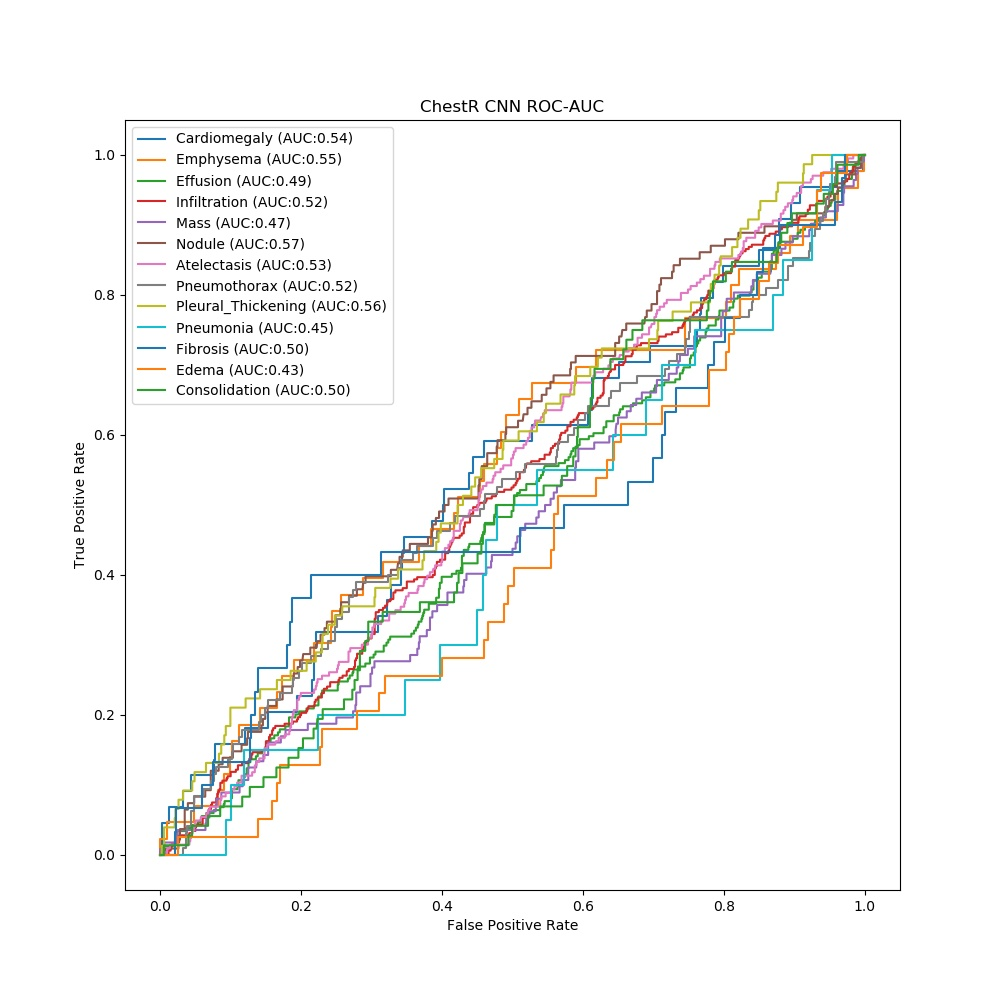
\includegraphics[width=\linewidth]{./images/chestr-cnn_roc_auc.jpg}
        \caption{CNN ROC AUC}
        \label{fig:cnn-roc-auc}
    \end{figure}

    For validation we can see from the the figure \ref{fig:cnn-samples-predictions} the model has learned some probability values for each of the disease, however these values are fairly low(less than 0.5). This doesn't really tend well for performing predictions on the data for which we do not have the diagnosis. It will be hard to predict exactly which disease is affecting these X-rays. 
    
    \begin{figure}
        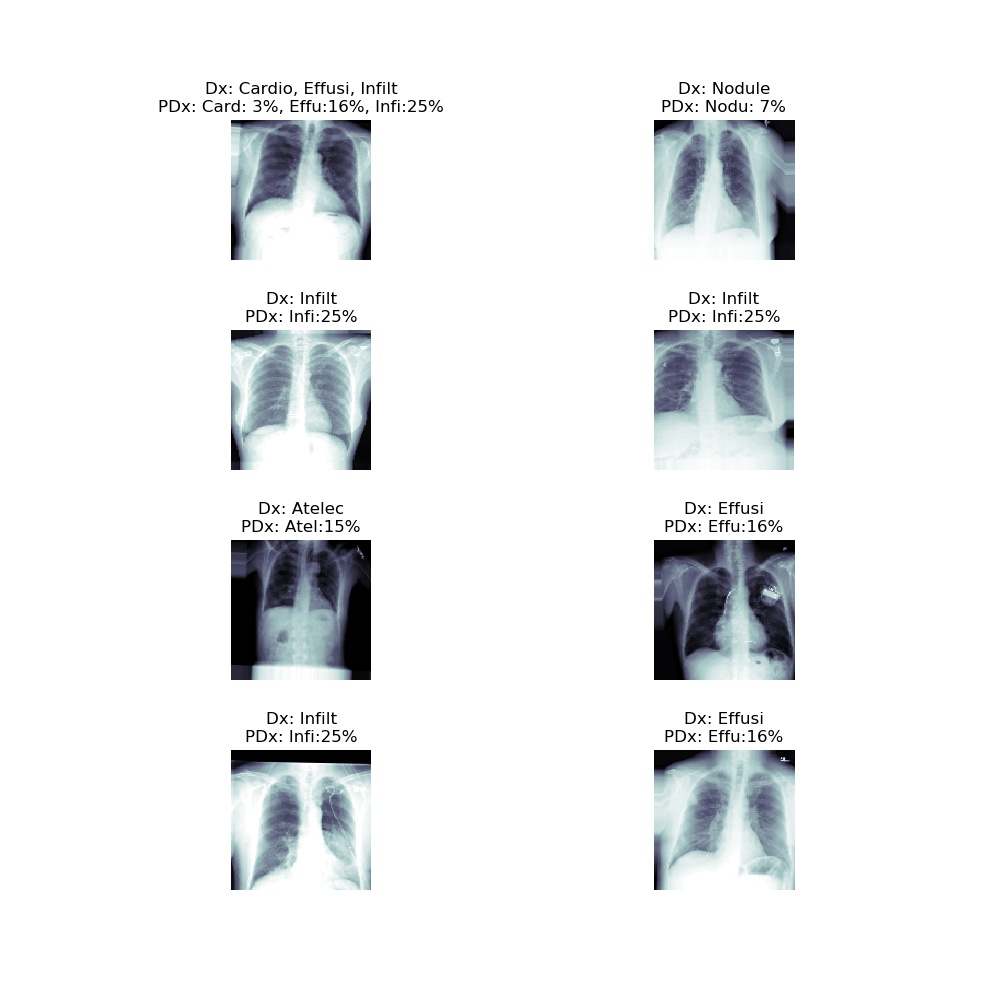
\includegraphics[width=\linewidth]{./images/chestr-cnn_sample-images-pred-view.jpg}
        \caption{CNN Sample images for disease predictions}
        \label{fig:cnn-samples-predictions}
    \end{figure}

    However, starting from the benchmark model, this is fairly positive direction towards predicting the disease labels. In any case this model performs a bit better than the benchmark on ROC - AUC metrics. 

    The VGG19 trained CNN model shows the following values for Precision and recall, and it can be seen that this is indeed performing "High Recall and low precision" thus the high values for prediction probabilities seen above.

    \begin{center}
        \begin{tabular}{||c c c c||}
            \hline
            Category&precis&recall&f1-score \\ 
            \hline
            Healthy&0.94&0.4&0.56 \\
            Cardiomegaly&0.06&0.63&0.12 \\ 
            \hline
            Healthy&0.95&0.92&0.93 \\
            Emphysema&0.04&0.06&0.05 \\ 
            \hline
            Healthy&0.5&0.01&0.02 \\
            Effusion&0.23&0.97&0.37 \\ 
            \hline
            Healthy&0&0&0 \\
            Infiltration&0.3&1&0.46 \\ 
            \hline
            Healthy&0.89&0.35&0.5 \\
            Mass&0.1&0.63&0.17 \\ 
            \hline
            Healthy&0.89&0.68&0.77 \\
            Nodule&0.1&0.31&0.16 \\ 
            \hline
            Healthy&0.82&0.28&0.42 \\
            Atelectasis&0.19&0.73&0.31 \\ 
            \hline
            Healthy&0.9&0.21&0.34 \\
            Pneumothorax&0.09&0.77&0.16 \\ 
            \hline
            Healthy&0.94&0.84&0.89 \\
            PleuralThic&0.05&0.15&0.07 \\ 
            \hline
            Healthy&0.98&0.82&0.89 \\
            Pneumonia&0.03&0.2&0.05 \\ 
            \hline
            Healthy&0.97&0.85&0.91 \\
            Fibrosis&0.03&0.15&0.05 \\ 
            \hline
            Healthy&0.96&0.91&0.93 \\
            Edema&0.01&0.03&0.02 \\ 
            \hline
        \end{tabular}
    \end{center}

    \section{Justification and Improvements}
    As can be seen from the figures \ref{fig:base-mlp-roc} \ref{fig:cnn-roc-auc} and \ref{fig:cnn-vgg19-roc-auc}, the non-transfer learning CNN model performs much better than our benchmark model. In fact it conservatively predicts the diseases, which though not satisfactory for any real life application is still on the right path to be experimented and improved. The fine tuning of the CNN model with the transfer learning was a failure. There needs to be more analysis done for figuring out why the application of transfer learning did not work. It is possible to seggregate the data and build individual models to predict the disease probability rather than counting and trying to predict these diseases together. 

    There is a scope of improvement in training the pretrained models. There are a few existing kernels that can be drawn on for some inspiration to improve the predictions on these models.\cite{cardio-kaggle}

    \section{Reflection}
    This has been quite a challenging problem, because it was the first time I had to deal with building a trainig model from scratch. The requirement gathering and challenges have been interesting. Quite a lot of research went into building a simple model itself and applications of machine learning in such fields have been eye opening. I would say this project although not a resounding success in implementing a very well predicting model provided enormous learning opportunity with regards to the Deep neural networks and the APIs for developing such networks. Also, most challenging part was also to get the Tensorflow running on the GPU, but worth the effort for saving on training time. 

    \begin{thebibliography}{999}

        \bibitem{xray-details} \url{https://www.radiologyinfo.org/en/info.cfm?pg=chestrad}
        \bibitem{nih-kaggle} \url{https://www.kaggle.com/nih-chest-xrays/data/home} 
        \bibitem{nih-gov-xray-release} \url{https://www.nih.gov/news-events/news-releases/nih-clinical-center-provides-one-largest-publicly-available-chest-x-ray-datasets-scientific-community}
        \bibitem{nih-chest-xray-download} \url{https://www.kaggle.com/nih-chest-xrays/data/downloads/data.zip/3}
        \bibitem{chexnet} \url{https://arxiv.org/pdf/1711.05225.pdf}
        \bibitem{simple-xray-cnn} \url{https://www.kaggle.com/kmader/train-simple-xray-cnn}
        \bibitem{github-proj} \url{https://github.com/shishirx34/Udacity/tree/master/Machine%20Learning%20Engineer%20Nanodegree/chestray_capstone/src}
        \bibitem{cardio-kaggle} \url{https://www.kaggle.com/kmader/cardiomegaly-pretrained-vgg16}

    \end{thebibliography}

\end{document}